\input{../preamble.tex}

\SetDate[02/04/2026]
\reversemarginpar
\setlength{\marginparsep}{.5cm}

\begin{document}
\pagestyle{fancy}
\fancyhead[L]{Première}
\fancyhead[C]{\textbf{Évaluation blanche 2 — Dérivation}}
\fancyhead[R]{\today}

\null\vspace{-30pt}
Consignes particulières : 
\begin{itemize}[label=$\bullet$]
	\item 
	La calculatrice est {interdite}.
	\item
	L'évaluation fait \pageref{lastpage} pages. La somme des points est \total{points}.
\end{itemize}

\marginpar{[pts]}
\hrule

%\subsection*{Automatismes}



\exe{4,difficulty=0}{
	Considérons la fonction $f$ donnée graphiquement ci-dessous.
	\begin{enumerate}
		\item 
		Quel est le signe de $f(2)$ ?
		\item 
		Quel est le signe de $f'(-0,5)$ ?
		\item 
		Donner approximativement la valeur de $f'(1,8)$.
		\item
		La tangente à $\C_f$ en $x=1$ a pour équation $y=6,03 - 6,35x$.
		En déduire la valeur de $f'(1)$.
	\end{enumerate}

	\begin{center}
	\begin{tikzpicture}[>=stealth, scale=1]
	\begin{axis}[xmin=-1, xmax=4, ymin=-6, ymax=6, axis x line=middle, axis y line=middle, axis line style=-, grid=both, xtick distance = 1, minor tick num = 1, clip=false]
		\addplot[BLUE_E, very thick, domain=-1:4, samples=100] {10*e^(-x^2) + x - 5}  node[right] {$\C_{f}$};
		\addplot[RED_E, <->, thick, domain=.4:1.65, samples=2, xshift=0, yshift=.5pt] {6.03-6.35*x}  node[pos=1, right] {$y = 6,03 - 6,35x$};
	\end{axis}
	\end{tikzpicture}
	\end{center}

}{exe:tangente-graphique}{
}

\exe{3,difficulty=0}{
	La courbe représentative d'un fonction $f$ est donnée ci-dessous.
	Compléter son tableau de signes.

	\begin{multicols}{2}
	\begin{tikzpicture}[>=stealth, scale=1]
	\begin{axis}[xmin=-1, xmax=4, ymin=-6, ymax=6, axis x line=middle, axis y line=middle, axis line style=-, grid=both, xtick distance = 1, minor tick num = 1, clip=false]
		
		% (f')
		%\addplot[myr, very thick, domain =-2:3, samples=50] {(x+1)*x*(x-2)+.5}  node[pos = .77, right=2pt] {$\C_{f'}$};
		\addplot[GREEN_E, very thick, domain=-1:4, samples=50] {10*e^(-x^2) + x - 5}  node[pos = 1, right] {$\C_{f}$};
	\end{axis}
	\end{tikzpicture}
	\hfill
	\vfill
	\begin{tikzpicture}
		\tkzTabInit
		 %[lgt=3,espcl=1.5]
	       		{$x$ / 1 , Signe de $f(x)$ / 2}
	       		{,,}
	\end{tikzpicture}
	\vfill\null
	\end{multicols}
}{exe:lecture-graphique}{
}




%\subsection*{Exercice}


\exe{3}{
	Donner la fonction dérivée de chaque fonction suivante.
	\begin{multicols}{2}
	\begin{enumerate}
		\item $f(x) = -8x^3 + 5x^2 - 57x + 219$
		\item $g(x) = 34x^3 +2x^2 +75x - 710$
	\end{enumerate}
	\end{multicols}
}{exe:derivation}{
}

\exe{4}{
	Développer et réduire chaque expression suivante.
	\begin{multicols}{3}
	\begin{enumerate}
		\item $f(x) = (3x+5)(5x+2)$
		\item $g(x) = 8x\left(\frac12x - \frac14\right)$
		\item $h(x) = -\frac12(x+9)(x-4)$
	\end{enumerate}
	\end{multicols}
}{exe:dev-red}{
}

\exe{6,difficulty=2}{
	Étudier la fonction $f$ donnée par
		\[ f(x) = -x^3 + 3x^2 + 9x - 5 \]
	pour des antécédents $x$ situés entre $-2$ et 4, en montrant d'abord que 
		\[ f'(x) = -3(x+1)(x-3) \]
}{exe:variations-d3}{
}


\begin{figure}[h]
	\centering	
	\begin{tikzpicture}
		\tkzTabInit
		 %[lgt=3,espcl=1.5]
	       		{$x$ / 1, Signe de $-3$ / 1, / 1, / 1, Signe de $f'(x)$ / 1, Variation de $f(x)$ / 2}
	       		{,,,,}
	\end{tikzpicture}
	\caption{Tableau de variations de $f$ et de signes de $f'$.}
	\label{fig:var-signe}
\end{figure}

\begin{figure}[h]
	\centering
	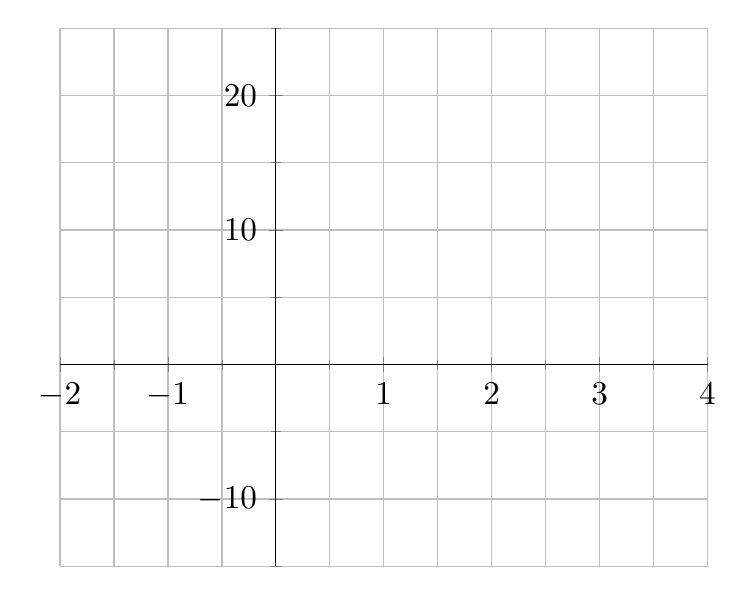
\begin{tikzpicture}[scale=1.2]
	\begin{axis}[
		xmin = -2, xmax=4,
		ymin=-15, ymax=25,
		axis x line=middle, 
		axis y line=middle, 
		axis line style=-,
		grid = both, % xlabel={$x$}, ylabel={$f(x)$},
		minor tick num = 1,
		clip=true,
	%xtick = {0, 0.2, ..., 1.4},
	%ytick = {-1, -0.5, 0, .5, 1.5},
	]
	\addplot[domain=-2:4, transparent, thick, samples=100] {-x^3 + 3*x^2 + 9*x -5} node[right]{$\C_f$};
	\end{axis}
	\end{tikzpicture}
	\caption{Graphe approximatif de $\C_f$.}
	\label{fig:Cf}
\end{figure}


%%%%%%%%%%%%

\label{lastpage}
\newpage
\fancyhead[C]{\textbf{Solutions}}
\shipoutAnswer

\end{document}
